\documentclass[article,dr=phil,type=drfinal,colorback,accentcolor=tud9c]{tudthesis}

\usepackage[english]{babel}
\usepackage{listings}
\usepackage{color}

\definecolor{mygreen}{rgb}{0,0.6,0}
\definecolor{mygray}{rgb}{0.5,0.5,0.5}
\definecolor{mymauve}{rgb}{0.38,0,0.38}

\lstset{ 
	backgroundcolor=\color{white},   % choose the background color; you must add \usepackage{color} or \usepackage{xcolor}; should come as last argument
	basicstyle=\footnotesize,        % the size of the fonts that are used for the code
	breakatwhitespace=false,         % sets if automatic breaks should only happen at whitespace
	breaklines=true,                 % sets automatic line breaking
	captionpos=b,                    % sets the caption-position to bottom
	commentstyle=\color{mygreen},    % comment style
	deletekeywords={...},            % if you want to delete keywords from the given language
	escapeinside={\%*}{*)},          % if you want to add LaTeX within your code
	extendedchars=true,              % lets you use non-ASCII characters; for 8-bits encodings only, does not work with UTF-8
	frame=single,	                   % adds a frame around the code
	keepspaces=true,                 % keeps spaces in text, useful for keeping indentation of code (possibly needs columns=flexible)
	keywordstyle=\bfseries\color{mymauve},       % keyword style
	language=Octave,                 % the language of the code
	morekeywords={*,get,await,deposit,interface},            % if you want to add more keywords to the set
	numbers=left,                    % where to put the line-numbers; possible values are (none, left, right)
	numbersep=5pt,                   % how far the line-numbers are from the code
	numberstyle=\tiny\color{mygray}, % the style that is used for the line-numbers
	rulecolor=\color{black},         % if not set, the frame-color may be changed on line-breaks within not-black text (e.g. comments (green here))
	showspaces=false,                % show spaces everywhere adding particular underscores; it overrides 'showstringspaces'
	showstringspaces=false,          % underline spaces within strings only
	showtabs=false,                  % show tabs within strings adding particular underscores
	stepnumber=1,                    % the step between two line-numbers. If it's 1, each line will be numbered
	stringstyle=\color{blue},     % string literal style
	tabsize=2,	                   % sets default tabsize to 2 spaces
	title=\lstname                   % show the filename of files included with \lstinputlisting; also try caption instead of title
}

\usepackage{ngerman}
\usepackage{float}

\newcommand{\getmydate}{%
  \ifcase\month%
    \or Januar\or Februar\or M\"arz%
    \or April\or Mai\or Juni\or Juli%
    \or August\or September\or Oktober%
    \or November\or Dezember%
  \fi\ \number\year%
}

\begin{document}
  \thesistitle{Evaluation of ABS in Modeling Real World Safety-Critical Systems}%
  {}
  \author{Chunyuan Yu}
  \birthplace{Liaoning}
  \referee{Clemens v. Loewenich}{Johannes Werner}[another one]
  \department{Fachbereich Informatik}
  \group{Software Engineering Group}
  \dateofexam{18. Juli 2018}{18. Juli 2018}
  \tuprints{12345}{1234}
  \makethesistitle
  \affidavit{Chunyuan Yu}
  
  \section{Introduction}
  
  This section gives an introduction for the whole thesis. It provides an overview of the cases to be studied, 
  
  \subsection{Overview}
  
  Nowadays, many modeling languages are used in the area of system modeling. Among them, the \textbf{Abstract Behavior Specification Language (ABS)} is well suited to model systems that are concurrent, distributed, object-oriented, built from components, and highly reusable []. As an actor-based and executable modeling language, ABS has been successfully applied in some scientific domains like railway operations [].
  
  In order to evaluate ABS as a modeling language for real world safety-critical systems, the Hybrid ERTMS/ETCS Level 3 Standard case study at ABZ 2018 from the railway domain with challenging safety requirements, and the Hemodialysis Machine case study at ABZ 2016 from the medical domain are chosen to be realized in ABS. The result will be compared to a model built in another modeling language to evaluate the ABS design.
  
  In more detail, in railway systems, to prevent accidents or congestions, it is meaningful to determine and control the location of trains. So a system model which manages the situation of the trains is of vital importance. In the medical area, some machines are used for therapy, such as, a hemodialysis (HD) machine, which helps clean the patients' blood. The machine should provide all features that a healthy kidney has, which is safety-critical. Therefore an appropriate system model should be built.
  
  \subsection{Motivation}
  
  The case study at ABZ 2018 issued from the railway domain focuses on the European Rail Traffic Management System (ERTMS) [], which aims to provide an integrated European railway system instead of several national train systems, in order to improve the capacity, safety and reliability. To increase the capacity of the railway with the Hybrid ERTMS/ETCS Level 3 specification, subparts of trackside detection sections called VSS (Virtual Sub-Sections) are used to stamp the train position information. To establish such a reliable railway system in ABS, it will be easier with the help of the management of VSS [].
  
  The case study at ABZ 2016 in the medical domain is concerned with the control of a HD machine. The HD machine is used to cure the kidney failure for patients, and has the functions to transport the patients' blood from and back to the patients' body with getting it filtered. During this process, the HD machine should be able to choose the exact type of therapy, do the therapy preparation including making sure of all the materials and parameters, do the therapy initiation and ending. Along with the procedure, both the general safety condition and software monitor function should be considered when building the whole HD system. 
  
  The primary objective of this Master Thesis is to implement the above two case studies in ABS, and to compare and discuss the effect of ABS design choices on the modeling process.
  
  \subsection{Sketch for the Structure of the Thesis}

  \begin{itemize}
  	
  	\item \textbf{Section 1. Introduction}
  	
  	The first part of the thesis mainly introduces the problems which are going to be solved in this thesis, and provides a sketch for the solution and discussion. 
  	
  	\item \textbf{Section 2. Background Knowledge}
  	
  	This section provides some background knowledge about the ABS modeling language, which is going to be evaluated in this thesis.
  	
  	\item \textbf{Section 3. Introduction of Case Study I: The Hybrid ERTMS/ETCS Level 3 Specification}
  	
  	Section 3 gives a detailed introduction of the Hybrid Level 3 specification. This part serves as a documentation part for case study I.
  	
  	\item \textbf{Section 4. Details of the Train Model for Case Study I}
  	
  	Section 4 analyzes the train model for case study I. It mainly explains the train model according to different VSS status and different types of trains. Later in this section, an extended discussion on the related properties from both static and dynamic point of view is given. 
  	
  	\item \textbf{Section 5. Case Study II:}
  	
  	\item \textbf{Section 6. Discussion and Evaluation}
  	
  	In the very last part of this thesis, according to all the above results, a discussion and evaluation is argued based on the provided test cases. It should be inspected if the ABS model provides an appropriate way to build the system, and the effect of design results.
  
  \end{itemize}	

  
  \section{Background Knowledge}
  
  This section simply introduces some background knowledge for this thesis. In the following, subsection 2.1 gives an introduction of ABS language, which is the main tool used for the two case studies in this thesis.Ans subsection 2.2 provides the reasons why ABS is chosen to be evaluated as the modeling language for real world safety-critical system cases.
  
  \subsection{Introduction of ABS Language}
  
  With the development of information technology, virtualized environment becomes a popular trend. People set up clouds to operate and control softwares, which makes it important to keep them distributed but concurrent. In order to develop modern softwares which are suitable for the above characters, a new software modeling language, ABS, is born for automation of the software engineering process.
  
  ABS (Abstract Behavioral Specification) language is a newly developed modeling language at an abstract level. It solves the problem about the architecture of softwares between the design and implementation part as a modeling language. ABS is actor-based and has many features, which are listed as follows:
  
  \begin{itemize}
  	
  \item \textbf{Immutable data and functions without side effect.}
  
  There are no public or private fields in ABS objects, so all data is defined just before being called. Functions in ABS have no side effect, which is good for model reasoning.
  
  \item \textbf{Smaller models.}
   
  Thanks to the user-defined data types, ABS models are smaller than the Java models which uses objects.)
  
  \item \textbf{Actor-based.}
  
  Processes are created by asynchronous calls, and are scheduled cooperatively. All processes run within one project.
  
  \item \textbf{Interfaces with methods to define behaviors.}
  
  This feature of ABS is similar to Java. They both use interfaces to specify object behaviors. The interfaces with corresponding methods are implemented by classes. One class can implement zero or more interfaces.
  
  \item \textbf{Safe concurrency.}
  
  Concurrency is a prominent characteristic of ABS. Since data types are immutable, and functions have no side effect, processes can be scheduled cooperatively. They have no influence on the states of other processes. This is extremely meaningful when checking for the existence of deadlocks.
  
  \item \textbf{Distributed and parallel computing.}
  
  With the quality of concurrency model and asynchronous method calls, it is easy to realize algorithms and modeling for distributed and parallel systems.
  
  \item \textbf{Formal semantics.}
  
  Tools used for program analysis are developed for ABS. Such as deadlock checker, resource analysis, simulator Erlang, and so on. []
  
  \item \textbf{Close-to-the-metal programming.}
  
  ABS is designed as a modeling language instead of a systems programming language.
  
  \end{itemize}

  As stated in the important feature ``actor-based'', ABS supports asynchronous method calls, and they generate new processes and run them cooperatively in one target. 
  
  To be more specific, for example, when one process, as the caller, starts an asynchronous method call, another process, as the callee, is created. Both of the processes can run at same time without interrupting each other, while each of them belongs to different Concurrent Object Groups (COGs) (COG is a kind of tool used on concurrent objects to cooperate concurrent tasks and their dependencies, like JCoBox in Java). When the caller needs the result of the callee, the caller may suspends itself and awaits, until the callee returns the result it needs. Then the caller process is awaken, the corresponding COG is activated again, and it goes on running. During this procedure, both the caller and callee are executed concurrently. With the use of COG, process in ABS can achieve the management of concurrency in an easy way.
  
  The above example can also be expressed in the following ABS code in Figure 1.
  
  \begin{figure}[H]
  	\begin{lstlisting}
  	Fut<Unit> f = o!m(a,b,c) ;
  	await f? ;
  	f.get ;\end{lstlisting}
  	\caption[Caption for LOF]{ABS code for the above example.}
  \end{figure}  
  
  Figure 1 shows a piece of example code. It calls method m with 3 parameters a, b, and c. The running result of method m of object o is then stored in the future type variable f. The await statement suspends the current process until method m finishes calling and future f gets its return value.
  
  With the help of type ``future'', ABS can better handle the issues about concurrency between different processes, and provide a better design as a result of the feature ``actor-based''.
    
  \subsection{Reasons for choosing ABS as the modeling language}
  
  It is concluded from the characteristics of ABS language that, ABS has two advantages over other standard programming languages. Firstly, as ABS is a feature-rich language, code written in ABS can be reused based on its features, which makes it possible to apply different features or components to different products. Secondly, ABS is designed using formal methods. It has formal semantics and is possible to be analyzed in formal ways, which can perform mathematical analysis and therefore provide better reliability, scalability, and integrity. []
  
  Besides the above two advantages, ABS also has its most important actor-based characteristic, which is of vital importance for measuring concurrent behaviors between processes. Unlike other common programming languages, ABS shows a great potential of concurrency. Nowadays, with the quick development of the scale of the enterprises and data storage and management, those systems in commercial or industrial areas are requested to be able to maintain large amount of applications running in parallel. This makes it urgent to widely apply the concepts of distributed software systems. With distributed systems, people can maintain computers and softwares from a remote control point. So it needs less efforts and resources than just managing them from exactly the same system, which may be enormous and waste a lot of resources. But the only skeptical problem is that, whether or not the softwares are running concurrently with each other. If they are not concurrent, some of the running progresses may be in an incorrect order, which may finally lead to an incorrect result. Just take the daily used bank account management issue as an example. If a person, as a client, holds a bank account with 500 Euros, and he deposits another 200 Euros into his account so that he can buy a 700 Euros computer from a server. Obviously, the action of deducting money from his bank account by the server should be made after the 200 Euros are booked in the bank account, or this transaction may fail. For the purpose of doing this, the code presents in Figure 2 can be used to get the actual account balance after depositing the 200 Euros.
  
  \begin{figure}[H]
  	\begin{lstlisting}
  	Fut<Int> f = o!deposit(500,200) ;
  	await f? ;
  	Int balance = f.get ;\end{lstlisting}
  	\caption[Caption for LOF]{ABS code for the bank account example.}
  \end{figure}
  
  After updating the actual account balance, a deduction can be done correctly.
  
  So, as mentioned above, ABS makes a great profit on concurrency. It is an object-oriented programming language like Java and Scala, and it is also an executable modeling language with actor-based characteristic.
  
  And also, ABS as a novel modeling language, it has a new type --- future. Futures are used to make synchronizations and get the result of another process as introduced above. It is really useful and convenient in system modeling area. In the following case studies, more details can be shown.
    
  
  \section{Introduction of Case Study I: The Hybrid ERTMS/ETCS Level 3 Specification}
  
  This section mainly introdces the background documentation specific for Case Study I: The Hybrid ERTMS/ETCS Level 3 Specification. Section 3.1 gives a basic introduction for ERTMS/ETCS, while section 3.2 provides a deeper understanding of the specification will be referred to in the following case study process.
 
  \subsection{Background knowledge of ERTMS/ETCS}
  
  The European Union (EU) is made up of 28 countries. There are many communications and collaborations happening among them every day. From the perspective of transportation, it is really helpful and important to build a seamless railway system for all the European countries, which can not only increase the capacity of a single railway system, but also provide a management method with better safety. In order to build the railway system among all the countries inside European Union as mentioned above, the European Rail Traffic Management System (ERTMS), regarded as a standard of management for the railway interoperation inside EU, is designed in response to such conditions. It is a standard that combines different national railway systems together to make an integrated railway system seamlessly as a whole, providing higher reliability and stability.
  
  According to the above requirements, three levels of ERTMS are developed:
  
  \begin{itemize}
  	
  \item \textbf{Level 1} provides a non-continuous communication between the train and trackside detection equipment by Euro-balises. Trackside equipment (to determine train integrity) and lineside signals are marked as necessary.
  
  \item \textbf{Level 2} provides continuous communication between the train and trackside detection equipment by the Global System for Mobile Communications Railway (GSM-R). Trackside equipment is necessary for train integrity, while lineside signals are optional.
  
  \item \textbf{Level 3} provides also continuous communication between the train and trackside detection equipment. What is different from level 2 is that, neither trackside detection equipment nor lineside signal is still necessary. The integrity of the train is managed by the on-board Train Integrity Monitoring System (TIMS).
  
  \end{itemize}
  
  Due to the operational and financial reasons, it is difficult to configure all the trains with ERTMS and TIMS. As a result, this case study mainly focuses on a Hybrid Level 3 specification, which gives a solution with different types of train configurations, those are, ERTMS trains with TIMS, ERTMS trains without TIMS, and non-ERTMS trains. This Hybrid Level 3 Principle is developed in order to optimize the supervision process, and is regarded as the most advanced standard. It considers the management of fixed Virtual Sub-Sections (VSS), which make up of the whole trackside detection sections. The status of VSS are classified into ``occupied'', ``free'', ``ambiguous'' and ``unknown'' according to the train's type, train's position, and information collected by the trackside detection equipment.  
    
  \subsection{Contents of Hybrid ERTMS/ETCS Level 3}
  
  The Hybrid ERTMS/ETCS Level 3 Specification is using fixed virtual blocks (officially regarded as Virtual Sub-Section) to manage the location of a train, which may be configured with Train Integrity Monitoring System (TIMS) or without TIMS but with trackside train detection. There is also another type of train mentioned in Hybrid Level 3, which is non-ERTMS train. Since the non-ERTMS train does not fit with systems like TIMS or ERTMS, and it just occupies the whole trackside detection section where it locates, there will not be too much detailed introduction over this type of train. In the following, it is going to focus on both types of ERTMS train --- TIMS train and non-TIMS train.
  
  This section firstly provides an introduction on the normal Level 3 specification. Since Level 3 principle may not be very suitable to the situation for the case study, the Hybrid Level 3 specification is then proposed. This section also gives a detailed introduction for the Hybrid ERTMS/ETCS Level 3 specification.
  
  \subsubsection{The ERTMS/ETCS Level 3 specification} 
  
  Before having a deeper understanding of the Hybrid Level 3, it is better to have a look at the Level 3 specification first. In the Level 3, the trackside train detection provides the information about the train position and train integrity confirmation by calling the train separation function. The train separation function usually depends on characteristics like the train position and train integrity status. [] The advantage of ERTMS/ETCS Level 3 over Level 1 and Level 2 lies on a combination of both financial reasons and efficient reasons. On one hand, unlike Level 2, which has to use the trackside equipment for managing train integrity, Level 3 does not need the trackside equipment for all the trains anymore, since it provides trains fitted with TIMS which can control the train‘s integrity by itself. With the configuration of TIMS, a large branch of trackside train detection can be omitted. So, there is a remarkable decrease on the implementation and management cost of the trackside equipment. On the other hand, using trackside system instead of installing trackside equipment along the track, it is more convenient and easy to manage the whole tracking system as the train moves. This states also an improvement on the behavior and performance of the track system. As a result, the Level 3 is considered as a more comprehensive regulation as the former ones.
  
  But, every coin has two sides. As in Level 3, every train should be installed with TIMS, which makes it possible to get the necessary information of train's position and train's integrity status for the train separation function. But it is really ambiguous to determine the integrity for some kinks of trains. For example, for those trains with a lot of containers, once the train arrives a station, it may drop several containers, and then goes on for the next station. In this case, it is hard to find out whether the train is integrate or not, since the train's length changes, but it leaves with all things needed. And also, if not using trackside train detection to determine the related information about the train, then the trackside must keep having control over the information, such as the train's position and integrity status, continuously. But it cannot be sure if the connection between the trackside and the train works always fine. For example, when some containers are unloaded or reloaded to another direction; or even just due to the loss of connection. All in all, it is important to have a real-time observation over the state of the train. But lack of the trackside train detection, it is hard to achieve this goal reliably. As a result, the Hybrid Level 3 specification is proposed on the basis of Level 3, in order to improve Level 3 at its demerits.
  
  \subsubsection{The Hybrid ERTMS/ETCS Level 3 specification} 
  
  In the Hybrid Level 3 specification, it uses fixed virtual blocks, or to some extent, moving blocks. There are still a limited amount of trackside train detections used in Hybrid Level 3, which can help to get more precise information about trains than Level 3, since that those trains, which lose their connections to trackside in Level 3, can still be on the line in Hybrid Level 3, with the help of trackside train detections. It is very useful to protect the disconnected trains, and recover such trains from crashes. For those TIMS trains, it is more effective using Hybrid Level 3, as it provides better reliability and stability, especially in busy time and stations. When there are not so many trains, no TIMS ERTMS trains can be scheduled without staring at the integrity by the trackside train detection. This can be realized in a cheaper and more effective way than Level 3. But after all, Hybrid Level 3 aims to make its contribution mainly to those TIMS trains for better schedule plans.[]
  
  In Hybrid Level 3 specification, there are two most important terminologies which are widely referred to --- TTD (Trackside Train Detection) and VSS (Virtual Sub-Section). TTD is usually a section defined by trackside train detection system, which plays a significant role in detecting the related information, such as train’s location and integrity status, about the train on the track. One TTD is made up of several VSS. VSS is virtual sub-section, it is a sub-part of TTD. VSS status reflects the current information of the corresponding location. For example, if an integer TIMS train is located in the current VSS, then the status of this VSS is reported as “occupied”. But for other types of trains, the VSS status is much more difficult to determine. This will be introduced with the example model in the following.

  There are several crucial principles in Hybrid Level 3 which need to be paid attention to:

  \begin{itemize}
  	
  	\item 
  	As Hybrid Level 3 is based on and developed from Level 3, only Hybrid Level 3 and Level 3 specification shall be considered in this case study.
  	
  	\item
  	One TTD section consists of several VSS sections. Which means that, TTD sections can be divided into several VSS sections.
  	
  	\item
  	If there is no train on a TTD section, then this TTD section is reported as ``free'', and this information should be regarded as ``safe''. As a result, all VSS sections belong to this TTD section should also be reported as ``free''.
  	
  	\item
  	Train data reported from integer trains should also be regarded as ``safe''. 
  	
  	\item
  	TTD normally has two states: ``free'' and ``occupied'', despite the different types of trains. State ``free'' means that there is no train on the current TTD section, while state ``occupied'' means that there exists at least one train on the TTD section.
  	
  	\item 
  	VSS has in total four states: ``free'', ``occupied'', ``ambiguous'', and ``unknown''. In addition to the two states TTD has, VSS has also another two states for measuring all situations. State ``ambiguous'' stands for a situation, where the current VSS is occupied by a train, but it is not sure if there is another train on the same VSS. State ``unknown'' means that, it is unknown, if the current VSS is occupied or free. []
  	
  \end{itemize}
  

  \section{Details of the Train Model for Case Study I}
  
  Based on the Hybrid ERTMS/ETCS Level 3 Specification, three kinds of trains are described in this train model. The first one, also the most common one, is TIMS-equipped ERTMS train (also known as Integer train), which precisely occupies the exact VSS it is in. The next one comes the ERTMS train not fitted with TIMS, which occupies the sections in the rear of the track, until the end of the trackside detection section. The last type mentioned in this train model is non-ERTMS train, which occupies the whole trackside detection section as soon as it appears on the track.
  
  This section provides some details about the train model written in ABS language for case study I. Firstly it states the status transformation among each VSS. Then it analyzes the model by comparing the above different types of train in order to verify the effectiveness of the process. At last it shows some extended discussion on the related properties of the model.
  
  \subsection{Status Transition among VSS}
  
  In order to determine the status of VSS, it is necessary to have the information of the TTD occupancy and the reports of train positions. []
  
  In the last section, four VSS states in Hybrid Level 3 are introduced. Each VSS is in one state at a time. A detailed description of these four states are listed as follows:
  
  \begin{itemize}
  	
  \item \textbf{Free}
  
  The trackside train detection knows exactly that, there is no train on the current VSS. The status of this VSS is recorded as ``free''.
  
  \item \textbf{Occupied}
  
  The trackside train detection knows exactly that, there is an integer train on the current VSS, and there are no other train(s) rearwards on the same VSS. The status of this VSS is recorded as ``occupied''.
  
  \item \textbf{Ambiguous}
  
  The trackside train detection knows exactly that, there is a train on the current VSS. But the trackside knows not for sure, if there are other train(s) rearwards on the same VSS. The status of this VSS is recorded as ``ambiguous''.  
    
  \item \textbf{Unknown}  
  
  The trackside train detection does not have a clue, if there is a train on the current VSS. And the trackside knows not for sure, if the current VSS is free. The status of this VSS is recorded as ``unknown''.
  
  \end{itemize}

  The above four status can be transformed from one status to another. Assume that the initial state of all VSS is unknown. The transition among them can be expressed with the following Figure 3.
  
  \begin{figure}[H]
  	\begin{center}
  		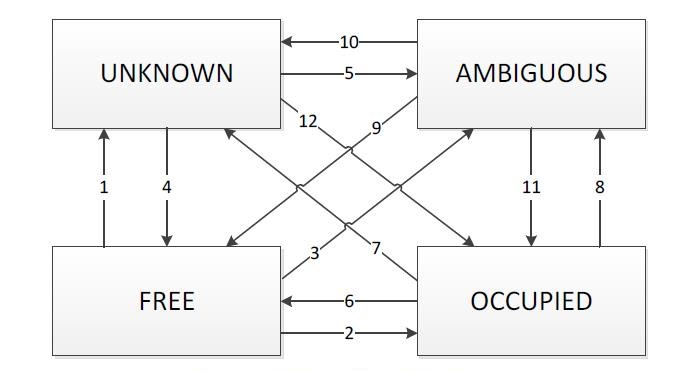
\includegraphics[width=0.5\textwidth]{fig3}
  		\caption[Caption for LOF]{Status Transition among VSS. []}
  	\end{center}
  \end{figure}

  As is known by default, TTD has two states, free and occupied. And VSS can be regarded as a sub-section of TTD. As a prerequisite, no matter what is the status of VSS, free or occupied or ambiguous or unknown, TTD can be occupied. But if TTD is free, then all the VSS belongs to this TTD are all free. Following is a detailed explanation for each status transition:
  
  \begin{itemize}
  	
  	\item \textbf{1 from free to unknown.}
  	
  	As the VSS state becomes unknown, there must be at least one train located on the current TTD, in the rear of the current VSS. So the status of TTD should be occupied. In this case, several circumstances should be considered:
  	
  	\begin{itemize}
  	
  	\item
  	
  	There may be a disconnected train on the track, and there is no information about whether the disconnected train has moved to the next TTD. So the status of current VSS should be unknown, until time is up, or the current TTD is made sure to be free, or the train is finally connected.
  	
  	\item 
  	
  	The old VSS status (free) may be sent to a train which is occurring a communication failure by its Movement Authority (MA), and now the train is longer located in the old VSS, which it was reported. Due to the communication failure, the VSS status should be set to unknown.
  	
  	\item 
  	
  	If there exists disconnection between the train and trackside detection, then the status of VSS could not be supervised by a normal way. Since the train can still move to next VSS after disconnection, the current VSS status should be set as unknown as soon as the ``disconnect propagation timer'' expires, until the current TTD is known as free, or the train is reconnected, or the disconnected part is connected on the previous TTD.
  	
  	\item 
  	
  	Based on the above situation, there is also another possible reason that, the current VSS is not part of the MA, which means that, the current VSS has no idea about how the train is moving. So it should be unknown to the VSS if the train is located on it.
  	
  	\item 
  	
  	There is a situation, that the train loses its integrity accidentally. This action calls an ``integrity loss propagation timer''. As long as the integrity-lost train is still on the current TTD, once the timer expires, the status of the last reported VSS should be marked as unknown.
  	
  	\item 
  	
  	There may be a disconnected train on the track, and there is no information about whether the disconnected train has moved to the next TTD. A propagation timer is set for this disconnected train since it disconnects. Not until the timer expires will the VSS status be unknown.
  		
    \end{itemize}	
  	
  	\item \textbf{2 from free to occupied.}
  	
  	\begin{itemize}
  		
  	\item 
  	
  	There is a train located on the current VSS, and the current status of the last VSS this train was reported is not unknown. As the train is moving in the right direction, the last VSS it was located in should also be reported with the status of ``occupied''.
  	
  	\item 
  	
  	If the train is moving from one TTD to the next TTD, and the TTD it has just left is now free, and the current VSS is the first VSS of the newly-entered TTD, then the VSS this train is currently located should be occupied.
  		
    \end{itemize}		
  		
  	\item \textbf{3 from free to ambiguous.}
  	
  	\begin{itemize}
	
	\item 
	
	There is a train located on the current VSS, but the trackside detection is not possible to determine that whether there are any other trains located in the rear of this connected train or not. The train should have connection with the trackside detection, since that, if the train gets disconnected, the status may be ``unknown'' instead of ``ambiguous''.
	
	\item 
	
    If the train is moving from one TTD to the next TTD, and the TTD it has just left is now free, and the current VSS is the first VSS of the newly-entered TTD, then the VSS this train is currently located should be not free. And if the integrity status of the train is lost or no information available, which means that it is impossible to make sure of the train is integrate or not, then the VSS status should be ambiguous.
	
    \end{itemize}  		
  	
  	\item \textbf{4 from unknown to free.}
  	
  	\begin{itemize}
	
	\item 
	
	Since the initial state of VSS is unknown, as long as it is confirmed that the current TTD has no train located on it, the current status of VSS is obviously free.
	
	\item 
	
	There is an integer train which loses its connection to the trackside detection, but reconnects at the same point. For this train, when its integrity is lost, the status of the VSS it is located becomes unknown. Then after reconnection, the VSS in advance of the train, which is also part of the original MA, becomes free.
	
	\item 
	
	There is an integer train which loses its connection to the trackside detection, but reconnects at the same point, and no change happens on the train data (including length). For this train, when its integrity is lost, the status of the VSS it is located becomes unknown. Then after reconnection, the VSS in the rear of the train, which is also part of the original MA, becomes free. And also, the subsequent VSS are still unknown at first, since the VSS, on which the connection-lost train is located, is free now.
	
    \end{itemize}  	
  	
  	\item \textbf{5 from unknown to ambiguous.}

  	\begin{itemize}
	
	\item 
	
	Due to disconnection or propagation of a train, the current status of VSS is unknown. So it is confirmed that there is at least one train on the track. But it is impossible for the trackside to confirm that if there are any other trains or vehicles located in the rear of a connected train. So the status of current VSS is turned into ambiguous.
	
    \end{itemize} 
   	
  	\item \textbf{6 from occupied to free.}
  	
  	\begin{itemize}
	
	\item 
	
	If there used to be a train located on the TTD, but now the train has left and TTD becomes free, then the current VSS also becomes free. Because that, information propagated from TTD is regarded as safe and trusted, which means that, TTD reports free, if and only if there is no train located on the current TTD. As a result, all VSS belong to this TTD can also be regarded as free.
	
	\item 
	
	If there is an integer train located on the VSS, then the VSS is occupied. When the integer train is reported to have left the VSS, then the status of the VSS is changed into free.
	
    \end{itemize}    	
  	
  	\item \textbf{7 from occupied to unknown.}
  	
  	\begin{itemize}
	
	\item 
	
	There must be train(s) located on the track, so VSS could be occupied. The current VSS is immediately turned into unknown as soon as the train located on the VVS disconnects from the trackside, which reveals that, there are still train(s) present, but due to disconnection, they cannot be detected. This may happen when the mute timer expires or it is end of a mission, which means the disconnection happens.
	
	\item 
	
    If an integer train is detected to be on the current VSS, then the status of the VSS is occupied. When the train has left the VSS, but meanwhile, it is reported as ``integrity lost'', or ``integrity information unavailable'', or train data has changed, then the status of the VSS should be changed. In this situation, the status of VSS should be set as unknown, since that, without having the integrity information of the train, it is unable to detect the location of the train, also the status of VSS. So the VSS, which is left by the train afterwards, should be set as unknown. The unknown state will be propagated until the disconnection timer expires or the train is reconnected or the whole TTD is confirmed to be free.
	
    \end{itemize}  
  	
  	\item \textbf{8 from occupied to ambiguous.}
  	
  	\begin{itemize}
	
	\item 
	
	If an integer train is detected to be on the current VSS, then the status of the VSS is occupied. When the train has left the VSS, but meanwhile, it is reported as ``integrity lost'', or ``integrity information unavailable'', or train data has changed, then the status of the VSS should be changed. In this situation, the status of VSS should be set as ambiguous, since that, without having the integrity information of the train, it is unable to detect the location of the train, also the status of VSS. And since the VSS is the train currently located on, the status of the current VSS should be ambiguous.
	
	\item 
	
	VSS is at first occupied, since at least one train is confirmed on the current VSS. If the VSS in the rear of the current VSS are all set to unknown, for example, when the train reconnects to the trackside detection, the VSS rearwards become unknown. If so, when the train leaves the current VSS, this VSS should be set as ambiguous, since that it is not possible for the trackside detection to get the information that whether there are other trains or vehicles in the rear of a connected train.
	
	\item 
	
	If there is another train also located on the VSS, but the trackside detection is not able to confirm that, then the status of the VSS should be set to ambiguous.
	
    \end{itemize}  
  	
  	\item \textbf{9 from ambiguous to free.}
  	
  	\begin{itemize}
	
	\item 
	
	Once the TTD information is confirmed, the status of TTD is regarded as trustable. So, if the TTD information reports that there is no train on the current track, then all the VSS belong to this TTD are also considered as free.
	
	\item 
	
    There may be a train, which has a vehicle rearwards. The vehicle may be either an exact train but without any connection to the trackside, or a virtual train which may lead to the ambiguous state of VSS, then this vehicle is considered as a shadow train. If the first train has already left the first VSS, the following VSS should be ambiguous because of the undetected shadow train. But after the detecting timer expires, these VSS can be reset to free.
	
    \end{itemize}  
  	
  	\item \textbf{10 from ambiguous to unknown.}
  	
  	\begin{itemize}
	
	\item 
	
	If there is a train which is not integrated, and the train may be on this VSS, the status of this VSS is ambiguous. After all those trains have left this VSS, and this information has been reported by TTD, the status of this VSS becomes unknown.
	
	\item 
	
	If there is a train which is not integrated, and the train may be on this VSS, the status of this VSS is ambiguous. If the train is not leaving, which means that the train may still be on this VSS, but the mute timer for the train is expired, or it is time to the end of mission, which means that the current location and state of this train is not available. Then the state of the current VSS should be unknown.
	
    \end{itemize}    	
  	
  	\item \textbf{11 from ambiguous to occupied.}
  	
  	\begin{itemize}
	
	\item 
	
	If there is a shadow train on the track, the trackside cannot detect it and starts a timer. Then, the status of the current VSS is ambiguous before the timer expires. Even though the shadow train may be leaving, as long as the leaving distance is shorter than the distance this train can move during the timer, the VSS status is still ambiguous. Once an integer train is reported on the current VSS after that, the status of the VSS should be occupied.
	
	\item 
	
	If there is a shadow train on the track, the trackside cannot detect it and starts a timer. Then, the status of the current VSS is ambiguous before the timer expires. If the TTD in the rear of the current train is free, and the current integer train on the same VSS has left the last TTD, then the current VSS should be occupied as the integer train is reported.
	
    \end{itemize}    	

  	\item \textbf{12 from unknown to occupied.}

  	\begin{itemize}
	
	\item 
	
	If there is an integer located train on a VSS, then the current TTD should report occupied. If the train disconnects and then reconnects within the same session with all the train data unchanged, then the current VSS should change its status from unknown (disconnection) to occupied (reconnection). As the same time, all the subsequent VSS also become unknown since that, once the train loses its connection, there is an integer train located on an occupied TTD, so the status of the rest VSS become unknown.
	
	\item 
	
	If there is an integer located train on a VSS, then the current TTD should report occupied. If the train disconnects from the trackside, then the current VSS becomes unknown. But as the train is still moving, once it arrives the next VSS, but that VSS has not received the disconnected information about the integer train, then this VSS will be considered as occupied first.
	
    \end{itemize}  

  The above are the detailed explanation of the state transformation among all the four states of VSS. In the next subsections, a concrete example as the train model build in ABS language will be displayed and analyzed. This will be shown as a further exploration of the concrete train model.
  
  \end{itemize}
  
  \subsection{TIMS-equipped ERTMS train (an integer train)}
  
  In the train model, the train comes first is an integer train, also known as TIMS-equipped ERTMS train. This kind of ERTMS train is fitted with TIMS, which means that it is responsible for its integrity. TIMS-equipped train use VSS to confirm the moving process and current situation of itself.
  
  In order to model this train, two interfaces are set up. One is interface VSS, which is used to confirm the situation of train according to the virtual fixed block it is located. The other one is interface RBC, which is used to implement the trackside system RBC to help propagate information between the train and the VSS.
  
  To confirm the status of VSS and TTD, it is necessary to modify the moving phase of the train. To achieve this goal, method leave and arrive are used to control the behavior of the train and further its influence on the status of VSS and TTD, while method send and receive are used for RBC to get and propagate information from the train and to other VSS. Figure 4 shows a piece of sample code:
  
  \begin{figure}[H]
  	\begin{lstlisting}
  	interface VSS {
  	Unit leave1(Int m, VSS vss, Int n1, Int n2) ;
  	Unit arrive1(Int m, Int n1) ;
  	}  	
  	interface RBC {
  	Unit receive1(Int m, VSS vss, Int n2, Int n3, RBC rbc) ;
  	Unit send1(Int m, Int n1, RBC rbc) ;
  	}\end{lstlisting}
  	\caption[Caption for LOF]{Sample ABS code for the TIMS-equipped ERTMS train.}
  \end{figure}
  
  The particular steps about the TIMS-equipped train's moving procedure is shown in Figure 5.
    
  \begin{figure}[H]
  	 \begin{center}
  	 	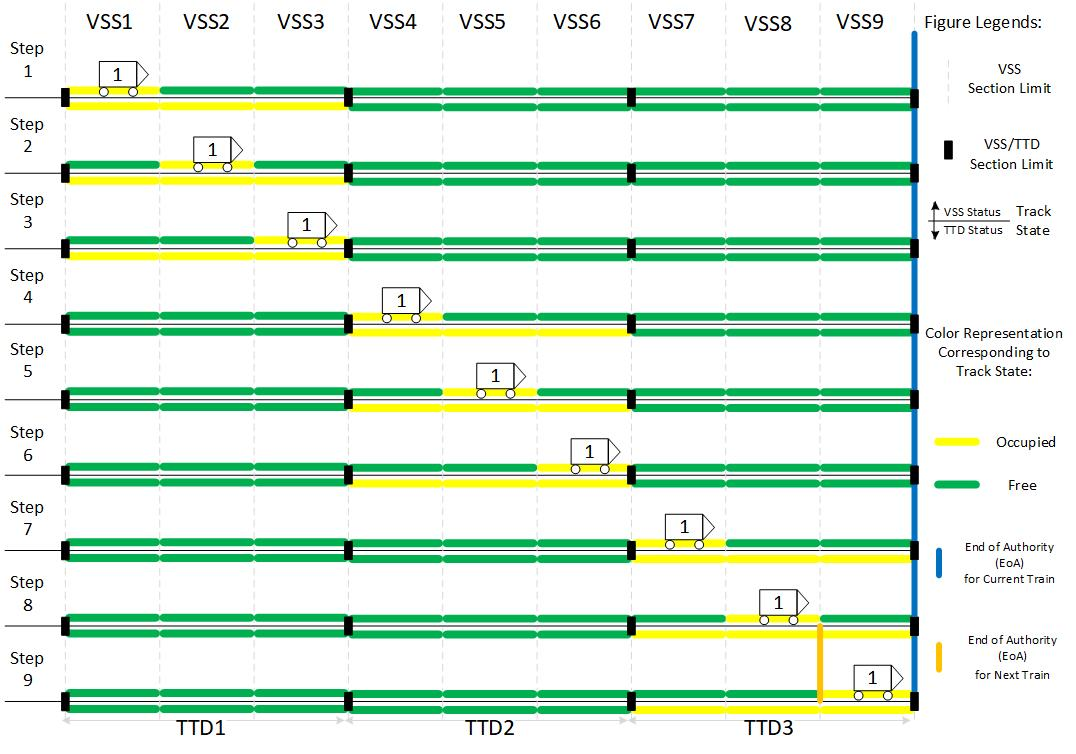
\includegraphics[width=0.5\textwidth]{train1}
  	 	\caption[Caption for LOF]{TIMS-equipped ERTMS train (an integer train).}
  	 \end{center}
  \end{figure}

  Train 1 in Figure 5 is a TIMS-equipped train. Here in the model in this situation, it holds its integrity all the time when it is moving. In this model, it is assumed that, all the trains are travelling in the same direction (from left to right in the figure) and in a straight line. Each TTD is made up of 3 VSS, and as shown in the figure, 3 TTD (9 VSS) are abstracted in this model. The EoA of the first train is set to the end point in the figure, which is VSS9.

  As shown in Figure 5, train 1 starts moving from VSS1, and stops at its End of Authority (EoA), which is VSS9. During its moving process, train 1 monitors the train integrity by itself as it is a TIMS-equipped train. The details of what happens and why it happens in each step are explained as follows:
  
  \begin{itemize}
  	
  	\item \textbf{Step 1}
  	
  	A TIMS-equipped train, train 1, enters the track. This changes the status of VSS1 from free to occupied, as mentioned above in the status transition. Since train 1 is located on TTD1, the state of TTD1 is turned into occupied from free. No changes to the other parts of the track.
  	
  	As soon as train 1 occupies VSS1, the trackside detection system RBC gets the information, that train 1 arrives and occupies VSS1. Then RBC sends this information back to the other VSS, informing the latest status of VSS1 and TTD1.
  	
  	\item \textbf{Step 2}
  	
  	Train 1 is moving, it leaves VSS1, and arrives VSS2. This action makes the status of VSS1 from occupied back to free, and VSS2 from free to occupied. Since train 1 is still located on TTD1, the state of TTD 1 remains occupied.
  	
  	As train 1 is moving, the RBC is also receiving information from train 1. When train 1 leaves VSS1 and arrives VSS2, RBC receives this information, and sends back the changes in the state of VSS1 and VSS2 to the other VSS. The status of TTD 1 remains unchanged. 	
  	
  	\item \textbf{Step 3}
  	
  	Train 1 leaves VSS2, and keeps moving. Then it arrives VSS3, the last VSS of TTD1. Train 1 sends its information about its location to the trackside system RBC, and then RBC sends back the information it knows about the states of the track back to the VSS.
  	
  	In step 3, the integrate train 1 is on VSS3, VSS2 is no longer occupied, VSS3 is occupied instead. TTD1 is still occupied.
  	
  	The following Figure 6 shows a piece of the output for train 1 between VSS2 and VSS4.
  	
  	\begin{figure}
  		\begin{center}
  			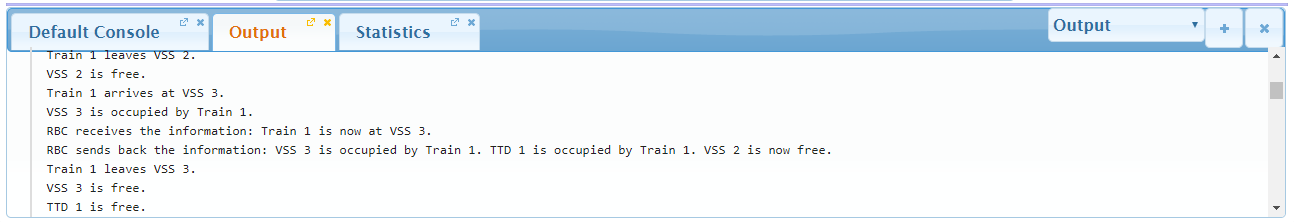
\includegraphics[width=0.8\textwidth]{fig6}
  			\caption[Caption for LOF]{Output for Train 1 between VSS2 and VSS4.}
  		\end{center}
  	\end{figure}
  	
  	\item \textbf{Step 4-6}
  	
    This part is almost the same as step 1-3. So it is omitted.
  	
  	\item \textbf{Step 7}
  	
  	When train 1 leaves VSS6, the status of VSS6 becomes free again, at the meantime, the state of TTD2 also becomes free, since that there is no train on TTD2 any more. Then train 1 arrives VSS7, which makes the status of VSS7 to be occupied. TTD3 is also occupied. This information is also reported to RBC, and then propagated to other VSS by RBC.
  	
  	\item \textbf{Step 8}
  	
  	Train 1 leaves VSS7 and keeps moving. VSS 7 is free again. Once train 1 is detected to be arriving at VSS8, VSS8 is occupied. TTD3 is still occupied. All the information are reported to and from RBC.
  	
  	\item \textbf{Step 9}
  	
  	As is set at the beginning of the program, the End of Authority for train 1 should be VSS9, which means that, the farthest VSS that train 1 can arrive is VSS9. So after leaving VSS8 and arriving VSS9, train 1 should stop at VSS9, and sets the EoA for next train to VSS8, since VSS8 is the farthest VSS that the next train can arrive. Then it reports its location, the latest VSS status and the new EoA information to RBC. RBC then propagates this information back to the other VSS. The simulation of the movement of train 1 ends here. The final status of VSS1-VSS8, TTD1 and TTD2 are free, VSS9 and TTD3 are marked as occupied.
  	 	
  \end{itemize} 
  
  \subsection{ERTMS train not fitted with TIMS}
  
  The second train in the model is an ERTMS train without TIMS. If an ERTMS train is not fitted with TIMS, then it needs a limited amount of trackside detection to help with getting the information about the train data, and some separation operations as well.
  
  \begin{figure}[H]
	\begin{lstlisting}
	Unit move() {
	Fut<Unit> fut1 = vss2!leave1(m,vss1,n1,n2) ;
	await fut1? ;
	fut1.get ;
	Fut<Unit> fut2 = vss2!receive1(m,vss1,n1,n2,rbc) ;
	await fut2? ;
	fut2.get ;
	
	//integrity loses
	
	//integrity loss propagation timer starts
	Time t = now() ;
	await duration(1,1) ;
	
	//integrity of the first half of Train 2 is confirmed
	
	Fut<Unit> fut3 = vss3!leave2(m,vss2,n2,n3) ;
	await fut3? ;
	fut3.get ;
	Fut<Unit> fut4 = vss3!receive2(m,vss2,n2,n3,rbc) ;
	await fut4? ;
	fut4.get ;
	}\end{lstlisting}
	\caption[Caption for LOF]{Sample ABS code for the ERTMS train not fitted with TIMS.}
  \end{figure}
    
  Here in the model, it is assumed that train 2 steps into the track also from VSS1. It keeps moving integrally on the track until it arrives VSS5, where it supposes to split into two parts, with the first half still integrated but the second half disconnected from the trackside. After the separation of the train, the first half of train 2 keeps moving to the subsequent VSS as an integer train, while the second half of train 2 is still disconnected. The status of each VSS should be measured according to the location of every part of train 2.
  
  For train 2, the interface VSS and interface RBC are still used, but with several extra methods. The measurement of the behavior of train 2 and the status of every VSS are classified into two parts: before separation and after separation of train 2. Because it should not be considered as an integer train before the separation, and the first part of train 2, which goes on moving after separation, can be reconsidered as an integer train to simulate. As a result, based on the first train which has been modeled above with interface VSS and interface RBC, a suitable model for train 2 is developed.
  
  A sketch of the model for train 2 could be like the above displayed program in Figure 7.
    
  The following Figure 8 shows the steps when the second train, which is without TIMS, is moving onto the track.
    
  \begin{figure}[H]
	\begin{center}
		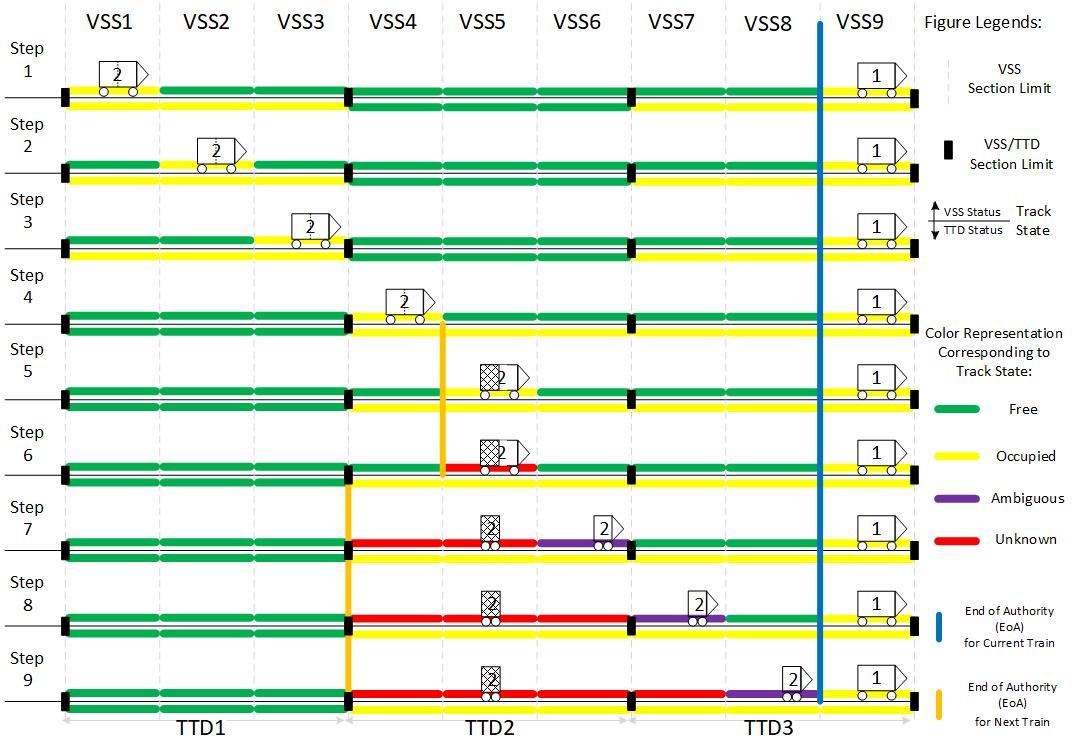
\includegraphics[width=0.5\textwidth]{train2}
		\caption[Caption for LOF]{ERTMS train not fitted with TIMS.}
	\end{center}
  \end{figure}

  The details of what happens and why it happens in each step are explained as follows:
  
  \begin{itemize}
	
	\item \textbf{Step 1}
	
    An ERTMS train not fitted with TIMS, train 2, enters the track. It should be noted that, train 1, which has stepped onto the track mentioned in the last part, is in front of train 2 and located on VSS9. The appearance of train 2 changes the status of VSS1 from free to occupied, as mentioned above in the status transition. Since train 2 is located on TTD1, the state of TTD1 is turned into occupied from free. No changes to the other parts of the track. 
    
    As soon as train 2 occupies VSS1, the trackside detection system RBC gets the information, that train 2 arrives and occupies VSS1. Then RBC sends this information back to the other VSS, informing the latest status of VSS1 and TTD1, which are both occupied.    
	
	\item \textbf{Step 2}
	
    Train 2 is moving, it leaves VSS1, and arrives VSS2. This action makes the status of VSS1 from occupied back to free, and VSS2 from free to occupied. Since train 2 is still located on TTD1, the state of TTD 1 remains occupied.
    
    As train 2 is moving, the RBC is also receiving information from train 2. When train 2 leaves VSS1 and arrives VSS2, RBC receives this information, and sends back the changes in the state of VSS1 and VSS2 to the other VSS. The status of TTD 1 remains unchanged, since train 2 is still on TTD1.

	\item \textbf{Step 3}
	
    Train 2 leaves VSS2, and keeps moving. Then it arrives VSS3, the last VSS of TTD1. Train 2 sends its information about its location to the trackside system RBC, and then RBC sends back the information it knows about the states of the track back to the VSS.
    
    In step 3, train 2 is on VSS3, VSS2 is no longer occupied, VSS3 is occupied instead. TTD1 is still occupied.
    
    \item \textbf{Step 4}
    
    Train 2 keeps moving. It leaves VSS3 and arrives at VSS4. It sends its location information to RBC, and RBC reports this information back to other VSS.
    
    It should be noticed that, since train 2 has left VSS3, TTD 1 and all VSS belongs to TTD1 are all free now.TTD 2 is now occupied.

    \item \textbf{Step 5-6}

    Train 2 stops at VSS5. This behavior is reported to RBC, and as a result, it also reports that the EoA for next train should be VSS4, as VSS4 is the last free VSS known to RBC. Then train 2 splits into two parts. The second half of train 2 is reported to lose its integrity, while the first half of train 2 still holds its integrity. According to the state transition specification introduced in section 4.1, the status of VSS5 becomes ambiguous due to the reported change for the integrity characteristic of train 2. Since the second half of train 2 loses its connection to the trackside, it is considered as remaining at VSS5 for now, while the first half of train 2 can still moving forward as an integer train.
    
    In step 6, when the first half of train 2 restarts moving, the status of VSS5 becomes unknown, since that it is unknown if the second part of train 2 is still at VSS5, or it moves as well. 
    
	\item \textbf{Step 7}
	
    As the first part of train 2 leaves VSS5, the status of VSS5 becomes unknown. According to the VSS state transition, since VSS4 is also part of TTD2, and TTD2 is now occupied by train 2, but it is unknown where the second part of train 2 is. So as the first part of train 2 moves forward, VSS 4 becomes unknown as well as VSS5. 
    
    When the first part of train 2 arrives at VSS6, the status of VSS6 is changed from free into ambiguous. The reason is that, the trackside RBC can get the information that the first part of train 2 is on VSS6, but it has no information about whether there is another vehicle (e.g. in this case, the second part of train 2 which has lost its integrity on VSS5.) in the rear of this first part of train 2 on the same VSS.
    
    It is also to be mentioned that, since VSS4 is now also reported as unknown, the latest EoA of the next train should be moved to VSS3.
    

    The following Figure 9 shows a piece of output for describing the influence train 2's behavior has over the status of the related VSS at its splitting point.
	
	\begin{figure}[H]
		\begin{center}
			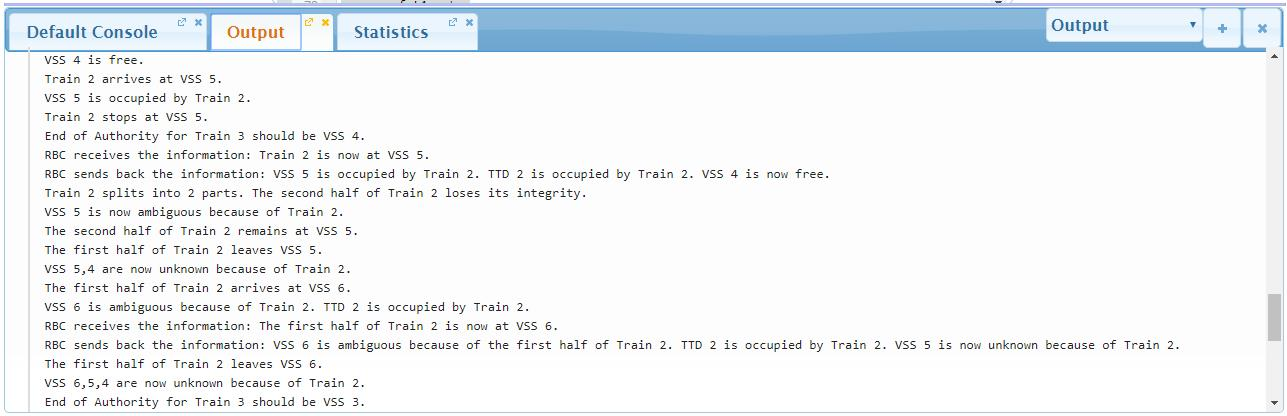
\includegraphics[width=0.8\textwidth]{fig9}
			\caption[Caption for LOF]{Output for Train 2 at VSS5 and VSS6.}
		\end{center}
	\end{figure}
	
	\item \textbf{Step 8}
	
	As the first part of train 2 keeps moving, it leaves VSS6 and heads to VSS7. It is not sure for RBC where exactly the first half of train 2 is, so VSS6 becomes also unknown. As a result, the whole TTD2 is occupied, while all the three VSS of TTD2 are unknown.
	
	When the first part of train 2 arrives at VSS7, the status of VSS7 becomes ambiguous, the reason is the same as mentioned before.
	
	\item \textbf{Step 9}
	
	Since train 1 stops at VSS9, and makes the EoA for train 2 be VSS8, the first half of train 2 arrives and stops at VSS8, with the status of VSS8 finally being ambiguous, and all VSS it passes after separation at VSS5 being unknown.
	
	To sum up, train 2 starts moving from VSS1, stops and splits at VSS5. After that, the second part of train 2 loses integrity, while the first part of train 2 keeps moving with integrity. Every VSS it arrives becomes ambiguous, and every VSS it then leaves becomes unknown, because of the unknown situation of the second part of train 2. The first part of train 2 finally stops at End of Authority, which is VSS8.
	
  \end{itemize}   
  
  \subsection{non-ERTMS train}
  
  The third train comes onto the track is a non-ERTMS train. According to the definition of non-ERTMS train, it occupies the whole trackside detection when it enters the track. On the basis of the above results from train 1 and train 2, it is reported that, only TTD1 and the three VSS belong to TTD1 are free, which means that, once train 3 appears on the track, TTD1, as well as VSS1-3, are occupied.
  
  \subsection{Extended Discussion on the Properties}
  
  This section mainly provides some extended discussions on the properties of the model. For example, about the deadlock analysis (SACO). Other analysis from both static and dynamic perspective will also be discussed.
  
  \subsubsection{Deadlock analysis}
  
  
  
  \subsubsection{Static analysis (safety)}
  
  
  
  \subsubsection{Dynamic analysis (runtime behavior)}
  
  
  
  
  
  \section{Case Study II: }
  
  \section{Discussion and Evaluation}














  \section{Generelle Informationen}
    Die Klasse basiert auf der \textaccent{tudreport}-Klasse von C. v. Loewenich und
    J. Werner. Alle "Anderungen dort wirken sich direkt auf die
    \textaccent{tudthesis}-Klasse aus. Genauer: die \textaccent{tudthesis}-Klasse definiert nur einige
    neue Befehle und legt die Formatierung der ersten zwei Seiten (Titelseite
    und R"uckseite des Titleblattes) fest. \textbf{Alle Vordefinierten Texte sind, wie verbindlich vorgeschrieben, in der hessischen Amtssprache
    gehalten\footnote{Deutschland hat (noch) keine Amtssprache.}.}

  \section{Verwendung der Klasse}
    Die Klasse wird verwendet, indem in der Dokumentenpr"aambel
    \textaccent{\textbackslash documentclass\{tudthesis\}}
    eingetragen wird.

  \subsection{Klassenoptionen}
    Die Klasse unterst"utzt alle Klassenoptionen der tudreport-Klasse.
    \paragraph{Neue Optionen}
    \begin{itemize}
      \item \textbf{type=<dr|drfinal|diplom|msc|pp|bsc|sta>}\\
        Hiermit wird die Art der Arbeit angegeben. Dies legt verschiedene
        Formatierungen fest.\\
        \begin{tabular}{ll}
        \textaccent{dr} &f"ur eingereichte Dissertationen\\
        \textaccent{drfinal} &f"ur genehmigte Dissertationen\\
        \textaccent{diplom} &f"ur Diplomarbeiten\\
        \textaccent{msc} &f"ur Master-Theses\\
        \textaccent{pp} &f"ur Project-Proposals\\
        \textaccent{bsc} &f"ur Bachelor-Theses\\
        \textaccent{sta} &f"ur Studienarbeiten
        \end{tabular}
      \item \textbf{dr=<rernat|ing|phil>}\\
        Hiermit wird die Art des Doktorgrads angegeben.\\
        \begin{tabular}{ll}
        \textaccent{rernat} &f"ur Dr. rer. nat.\\
        \textaccent{ing} &f"ur Dr.-Ing.\\
        \textaccent{phil} &f"ur Dr. phil.
        \end{tabular}\\
        F"ur den Fall, dass der gew"unschte Titel nicht vorhanden ist, gibt
        es den Befehl \textbf{\textbackslash drtext\{\#1\}}, wobei \#1 z.B.
        \glqq Zur Erlangung des Grades eines Doktors der
        Technischen Wissenschaften (Dr.\ rer.\ tech.)\grqq\ ist.
    \end{itemize}

  \subsection{Befehle}
    \begin{itemize}\itemsep-0.5\parsep
      \item \textbf{\textbackslash thesistitle\{\#1\}\{\#2\}}\\
        \#1: Titel der Arbeit in der Erstsprache (z.B. Deutsch)\\
        \#2: Titel der Arbeit in der zweiten Sprache (z.B. Englisch)
      \item \textbf{\textbackslash makethesistitle}\\
        Erzeugt die korrekte Titelseite
      \item \textbf{\textbackslash author\{\#1\}}\\
        \#1: Name des Autors
      \item \textbf{\textbackslash birthplace\{\#1\}}\\
        \#1: Geburtsort des Autors (bei Dr.-Arbeit verbindlich)
      \item \textbf{\textbackslash date\{\#1\}}\\
        Standard ist der aktuelle Monat und das aktuelle Jahr (z.B. \getmydate)\\
        \#1: individuelles Datum
      \item \textbf{\textbackslash referee\{\#1\}\{\#2\}[\#3]}\\
        Namen der Gutachter, (3. Gutachter optional)
      \item \textbf{\textbackslash department\{\#1\}}\\
        Fachbereich an dem die Arbeit durchgef"uhrt wurde. Standard ist
        \glqq Fachbereich Physik\grqq.
      \item \textbf{\textbackslash group\{\#1\}}\\
        Arbeitsgruppe / Institut an dem die Arbeit durchgef"uhrt wurde
      \item \textbf{\textbackslash dateofexam\{\#1\}\{\#2\}}\\
        \#1: Tag der Einreichung der Arbeit\\
        \#2: Tag der Pr"ufung / Tag des Abschlusses\\
        \textaccentcolor{Wird nur bei \textaccent{type=drfinal} verwendet.
        Ansonsten wird ein leeres Feld erzeugt, in das bei Abgabe der 
        Arbeit ein Stempel gesetzt wird.}
      \item \textbf{\textbackslash tuprints\{\#1\}\{\#2\}}\\
        \#1: \textaccent{<URN-ID>} aus \textaccent{urn:nbn:de:tuda-tuprints-<URN-ID>}\\
        \#2: \textaccent{<tuprints-ID>} aus \textaccent{http://tuprints.ulb.tu-darmstadt.de/<tuprints-ID>}\\
        Entspricht der Empfehlung auf der tuprints FAQ-Seite: \textaccent{http://tuprints.ulb.tu-darmstadt.de/faq.html\#urlreservation}
      \item \textbf{\textbackslash affidavit[\#1]\{\#2\}}\\
        \#1: Datum der Eigenst"andigkeitserkl"arung (optional)\\
        \#2: Signatur unter der Unterschrift
    \end{itemize}

\end{document}
